\chapter{Preparations to experiments}

\section{Choosing the correct configurations}

In order to receive a wide set of data from the measurements, tests should be
conducted using broad range of benchmark kernels with various classes sizes.
To break down the hierarchy of the test cases, it is a sound strategy to start
from the biggest piece $-$ the server. Computational nodes used for the 
experiments are server-grade machines, codenamed `sanna.kask' and
`vinnana.kask' respectively. Next step are the devices that the individual
benchmarks use during runs. Each node utilize three setting: `CPUs', `GPUs'
and the `Hybrid' benchmarks, which are combination of previous two. After
choosing the device, the correct implementation is specified, based both on
the currently used server and device. This way, it has been decided, that in
order to diversify the tests, implementation on the servers should vary.
Experiments on `sanna.kask' are utilizing the implementation based on OpenMP,
where the `vinnana.kask' server uses the solutions with MPI, TensorFlow and
Horovod. Based on the device utilized, implementation are either OMP-C++ or
MPI-Fortran for using on the CPUs and OMP-CUDA or Horovod-Python on GPUs.
Another parameter of the tests are the benchmarks, which are the short
applications or kernels, that solves various problems based on computational
fluid dynamics. The main goal of the benchmark is to evaluate the performance
of workstations by utilizing its targeted resources to the maximum. Properly
conducted tests should include various benchmarks in order to avoid bias on
the collected measurements data. The sets of used benchmarks are more complex
that the previously mentioned parts of the configuration and will be explained
graphically on the charts in the next section, but it should be mentioned, that
all implementation except Horovod-Python uses three different benchmarks with
various class sized. The Horovod-Python implementation use only one
application, the custom deep neural networks model. Finally, based on both
implementation and benchmark, the configuration is defined. By configuration
we should expect the resources used $-$ for the CPUs benchmark, such resources
are the CPUs themselves and their logical processors, and for the GPUs 
benchmarks $-$ the GPUs themselves and reserved for them CPUs threads. Again,
the amount of configurations set for the purpose of the experiments are
significant, therefore this part will also be represented in an easier to
understand, graphical way.

All the mentioned benchmarks fulfill the most important requirement, that is,
they utilize the targeted devices resources to the maximum or near-maximum.
Therefore, the next factor should be the execution time. It should be noted,
that this parameter is important, because of two reasons $-$ first, too short
benchmark kernel exposes the measurements to inaccuracy. To put this in
a~practical way, we should at first find the measurements tool with lowest
sampling rate, that is possible due to their implementation. In our case it is
the Yokogawa WT310E Power Meter $-$ its software, the Yokotool, enables the
measurements with the shortest interval of 0.1 second. Other methods, such as
Linux Perf and NVML should use this sampling frequency as well, in order to
maintain cohesion. In one of the research
papers~\cite{Performance_Energy_Aware_Optimization_Czarnul} that covered the
topic of energy awarness in parallel applications, authors discussed the
sampling period of \emph{nvidia-smi}, which is 1 second, and the execution
times of various benchmarks. Those values varied between 20 and 200 seconds,
which gives the maximal error of GPU power draw reading less than 5\% and the
minimal error for the longest test runs is less than 0.5\%.

\newpage

This insight gives us a simple formula:

\begin{equation} \label{eq:Error of power draw readings}
    E = \frac{x}{T} [\%]
\end{equation}

Where:

\begin{conditions}
    E & Error of reading $[\%]$ \\
    x & Lowest sampling rate of the measurements tool $[s]$ \\
    T & Execution time of benchmark $[s]$ \\
\end{conditions}

Based on that information, it has been tentatively accepted, that the maximum
error of power draw reading should be lower than 0.5\%, to be considered
satisfactory. With lowest possible sampling period of 0.1 second, the
execution time of any benchmark should be at least 20 seconds. To make sure,
that this constraint is satisfied at all times, the preliminary tests should
be done utilizing all of the resources on gives device, i.e. CPU benchmarks
should be run on all logical processors available in a parallel manner.
At last, benchmark kernel should be also short enough in order to avoid
excessively long execution time.

\section{Preliminary tests}

The goal of the set of preliminary tests is to choose three, best suitable
benchmarks from each implementation, based on the metrics stated earlier.

\begin{itemize}
    \item Implementation: \textbf{OMP-CPP}
    \begin{itemize}
        \item Benchmarks available: IS, FT, EP, CG, MG, LU, SP \& BT
        \item Class sizes to choose from: B, C \& D
        \item 24 different combinations of benchmarks and class sizes in total
        \item All tests were run on 2 CPUs and 40 logical processors in parallel
    \end{itemize}
    \item Implementation: \textbf{OMP-CUDA}
    \begin{itemize}
        \item Benchmarks available: IS, FT, EP, CG, MG, LU, SP \& BT
        \item Class sizes to choose from: C, D \& E
        \item 24 different combinations of benchmarks and class sizes in total
        \item All tests were run on a single GPU with the same grid sizes each time
    \end{itemize}
    \item Implementation: \textbf{MPI-Fortran}
    \begin{itemize}
        \item Benchmarks available: IS, FT, EP, CG, MG \& LU
        \item Class sizes to choose from: B, C \& D
        \item 18 different combinations of benchmarks and class sizes in total
        \item All tests were run on 2 CPUs and 32 logical processors in parallel
    \end{itemize}
    \item Implementation: \textbf{Horovod-Python}
    \begin{itemize}
        \item Benchmark available: XCeption
        \item Number of training epochs: 1, 3 \& 5
        \item 3 different combinations of model training parameters to choose from
        \item All tests were run in configurations with 1, 2 \& 4 GPUs, to
        check training behavior
    \end{itemize}
\end{itemize}

Every configuration stated above has been conducted 3 times in order to obtain
an average results, which are presented in the tables below.

\newpage

\begin{table}[!ht]
    \centering
    \small
    \caption{Execution times of OMP-CPP benchmarks}\label{tbl:table-label}
    \begin{tblr}{%
        hlines,%
        vlines,%
        row{1}={font=\bfseries},%
        column{1}={halign=c},%
    }%
        Benchmark & Class size & Execution time [s] & Benchmark & Class size & Execution time [s] \\
        IS & Class B & 0.35 & FT & Class B & 2.92 \\
        IS & Class C & 1.25 & FT & Class C & 16.14 \\
        IS & Class D & 37.53 & FT & Class D & 371 \\

        EP & Class B & 3.06 & SP & Class B & 14.48 \\
        EP & Class C & 11.96 & SP & Class C & (freezed) \\
        EP & Class D & 177 & SP & Class D & (core dumped) \\

        CG & Class B & 7.77 & BT & Class B & 15.82 \\
        CG & Class C & 27.2 & BT & Class C & 55.182 \\
        CG & Class D & (freezed) & BT & Class D & 1185 \\

        MG & Class B & 2.32 & LU & Class B & 9.88 \\
        MG & Class C & 17.459 & LU & Class C & 34.88 \\
        MG & Class D & 185 & LU & Class D & 1111 \\
    \end{tblr}
\end{table}


According to tests, three CPUs benchmarks has been chosen as the most suitable for
the main experiments on \emph{sanna.kask} later. Those benchmarks are:

\begin{itemize}
    \item \textbf{bt.C} $-$ Block Tri-diagonal solver, class size `C'
    \item \textbf{is.D} $-$ Integer Sort, class size `D'
    \item \textbf{lu.C} $-$ Lower-Upper Gauss-Seidel solver, class size `C'
\end{itemize}

\begin{table}[!ht]
    \centering
    \small
    \caption{Execution times of OMP-CUDA benchmarks}\label{tbl:OMP-CUDA}
    \begin{tblr}{%
        hlines,%
        vlines,%
        row{1}={font=\bfseries},%
        column{1,2,4,5}={halign=c},%
    }%
        Benchmark & Class size & Execution time [s] & Benchmark & Class size & Execution time [s] \\
        IS & C & (too short) & FT & C & 6.63 \\
        IS & D & 15.33 & FT & D & (unsuccesful) \\
        IS & E & (not defined) & FT & E & (unsuccesful) \\

        EP & C & (too short) & CG & C & (too short) \\
        EP & D & 27.16 & CG & D & (freezed) \\
        EP & E & 442.79 & CG & E & (freezed) \\

        MG & C & (too short) & LU & C & 16.89 \\
        MG & D & (unsuccesful) & LU & D & 300.74 \\
        MG & E & (unsuccesful) & LU & E & (unsuccesful) \\

        SP & C & 10.39 & BT & C & 12.19 \\
        SP & D & 220.86 & BT & D & (unsuccesful) \\
        SP & E & (unsuccesful) & BT & E & (unsuccesful) \\
    \end{tblr}
\end{table}

According to tests, three GPUs benchmarks has been chosen as the most suitable for
the main experiments on \emph{sanna.kask} later. Those benchmarks are:

\begin{itemize}
    \item \textbf{lu.D} $-$ Lower-Upper Gauss-Seidel solver, class size `D'
    \item \textbf{sp.D} $-$ Scalar Penta-diagonal solver, class size `D'
    \item \textbf{ep.D} $-$ Embarassingly Parallel, class size `D'
\end{itemize}
\newpage

\begin{table}[!ht]
    \centering
    \small
    \caption{Execution times of MPI-Fortran benchmarks}\label{tbl:MPI-Fortran}
    \begin{tblr}{%
        hlines,%
        vlines,%
        row{1}={font=\bfseries},%
        column{1,2,4,5}={halign=c},%
    }%
        Benchmark & Class size & Execution time [s] & Benchmark & Class size & Execution time [s] \\
        IS & B & 0.18 & FT & B & 3.11 \\
        IS & C & 0.8 & FT & C & 13.83 \\
        IS & D & 17.02 & FT & D & 360.15 \\

        EP & B & 1.11 & CG & B & 3.33 \\
        EP & C & 4.39 & CG & C & 8.57 \\
        EP & D & 71.16 & CG & D & 761.02 \\

        MG & B & 0.48 & LU & B & 10.97 \\
        MG & C & 4.5 & LU & C & 41.81 \\
        MG & D & 88.34 & LU & D & 770.52 \\
    \end{tblr}
\end{table}


According to tests, three CPUs benchmarks has been chosen as the most suitable for
the main experiments on \emph{vinnana.kask} later. Those benchmarks are:

\begin{itemize}
    \item \textbf{ep.D.x} $-$ Embarassingly Parallel, class size `D'
    \item \textbf{lu.C.x} $-$ Lower-Upper Gauss-Seidel solver, class size `C'
    \item \textbf{is.D.x} $-$ Integer Sort, class size `D'
\end{itemize}

\begin{table}[!ht]
    \centering
    \small
    \caption{Execution times of Horovod-Python benchmarks}\label{tbl:Horovod-Python}
    \begin{tblr}{%
        hlines,%
        vlines,%
        row{1}={font=\bfseries},%
        column{1,2,4,5}={halign=c},%
    }%
        Number of GPUs & Number of iteration & Execution time [s] \\
        1 & 1 & time \\
        1 & 3 & time \\
        1 & 5 & time \\

        2 & 1 & time \\
        2 & 3 & time \\
        2 & 5 & time \\

        4 & 1 & time \\
        4 & 3 & time \\
        4 & 5 & time \\
    \end{tblr}
\end{table}


According to tests, the best number of epochs for the training of `XCeption'
model is 1. Test accuracy of model is high and the execution time is
satisfactory.

What is worth noting in terms of GPUs benchmarks is the fact, that while
utilizing between 90$\sim$100\% fo the GPUs resources, various kernels results in
different power draw values. The averages of those values are listed below and
may provide an additional insight on the future experiments:

\begin{itemize}
    \item \textbf{lu.D} $-$ Power draw fluctuates between 200$\sim$230 [W]
    \item \textbf{sp.D} $-$ Average power draw of 200$\sim$210 [W]
    \item \textbf{ep.D} $-$ Average power draw of 155$\sim$160 [W]
    \item \textbf{XCeption} $-$ Average power draw of 180$\sim$185 [W]
\end{itemize}
\newpage

\section{Overview on all final configurations}

The measurements will be conducted on many different setups, therefore it is
important to explain throughly the entire hierarchy of the configurations.

% Servers:
\subsection{Servers}
The tests will be conducted on two computational nodes: \emph{sanna.kask}
and \emph{vinnana.kask}\@. Both of those machines have two Intel Xeon CPUs and
several NVIDIA Quadro RTX GPUs. Paired with huge amount of RAM, these servers
are suitable choices in terms of choosing the testbed machines.

\begin{figure*}[hbt!]
    \centering
    \captionsetup{width=.33\linewidth}
    \begin{minipage}[t]{0.33\textwidth}
        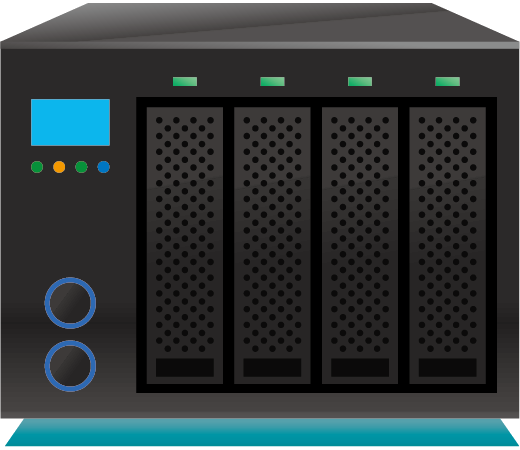
\includegraphics[width=\textwidth]{figures/servers/sanna.kask.png}
        \caption{sanna.kask}\label{fig:sanna.kask}
    \end{minipage}
    \hspace{3cm}
    \centering
    \captionsetup{width=.21\linewidth}
    \begin{minipage}[t]{0.21\textwidth}
        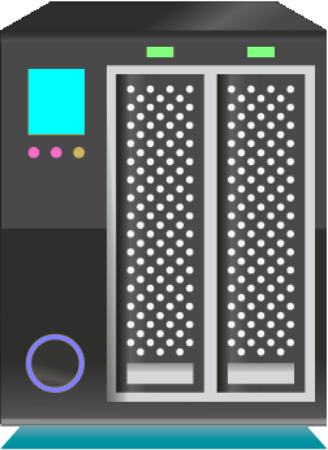
\includegraphics[width=\textwidth]{figures/servers/vinnana.kask.png}
        \caption{vinnana.kask}\label{fig:vinnana.kask}
    \end{minipage}
\end{figure*}

Despite the similarity between those two servers, their components slightly
differs from each other. A detailed comparison of their parts is listed in the
table below:

\begin{table}[hbt!]
    \centering
    \small
    \caption{Overview on components of the servers used in experiments}\label{tbl:Servers_components}
    \begin{tblr}{
        hlines,
        vlines,
        row{1}={font=\bfseries,halign=c,bg=lightgray!30},
    }
                & sanna.kask & vinnana.kask \\
        OS      & Linux Ubuntu 22.04 LTS & Linux Ubuntu 22.04 LTS \\
        CPUs    & {2 $\times$ Intel\@(R) Xeon\@(R) \\ Silver 4210 CPU\@ 2.20GHz, \\ TDP\@: 10/10 85 [W]}
                & {2 $\times$ Intel\@(R) Xeon\@(R)  \\ Silver 4210 CPU\@ 2.20GHz, \\ TDP\@: 10/10 85 [W]} \\
        GPUs    & {8 $\times$ NVIDIA Quadro RTX 6000, \\ VRAM\@: 24 GB, \\ power draw range: 100\@-260 [W]}
                & {4 $\times$ NVIDIA Quadro RTX 5000, \\ VRAM\@: 16 GB, \\ power draw range: 100\@-230 [W]} \\
        Motherboard & Inspur YZMB\-01130\-107 & Inspur YZMB\-01130\-107 \\
        RAM     & 384 GB, DDR4, 2400 (MHz) & 384 GB, DDR4, 2400 (MHz) \\
        PSUs    & 4 $\times$ Delta Electronics DPS-2200AB-2 & 4 $\times$ Delta Electronics DPS-2200AB-2 \\
    \end{tblr}
\end{table}

\newpage

% Devices:
\subsection{Devices}
Next, benchmarks will be organized based on devices,
that will be utilized during tests. On this level, we distinguish three
configurations: \emph{CPUs}, \emph{GPUs} and the \emph{Hybrid}, when both
are utilized during experiments. 

\begin{figure*}[hbt!]
    \captionsetup{width=.3\linewidth}
    \begin{minipage}[t]{0.3\textwidth}
        
\includegraphics[width=\textwidth]{figures/devices/Intel_CPU.png}
        \caption{CPUs benchmarks, utilizing the Intel Xeon Silver CPUs}\label{fig:Intel_CPU}
    \end{minipage}\hfill
    \captionsetup{width=.3\linewidth}
    \begin{minipage}[t]{0.3\textwidth}
        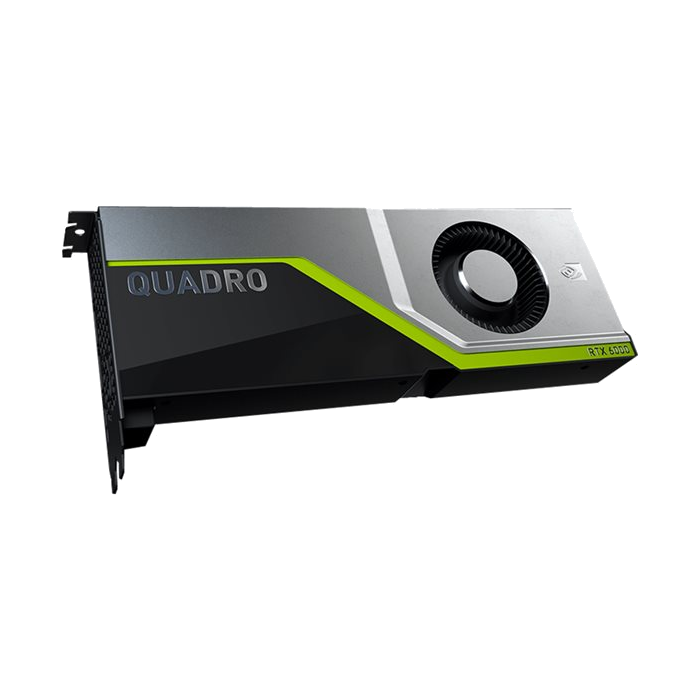
\includegraphics[width=\textwidth]{figures/devices/NVIDIA_GPU.png}
        \caption{GPUs benchmarks, utilizing the NVIDIA Quadro RTX GPUs}\label{fig:NVIDIA_GPU}
    \end{minipage}\hfill
    \captionsetup{width=.3\linewidth}
    \begin{minipage}[t]{0.3\textwidth}
        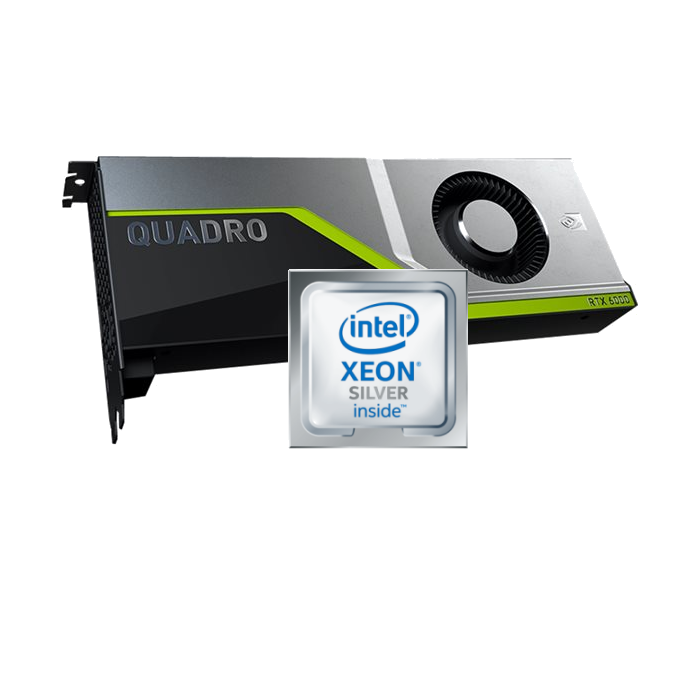
\includegraphics[width=\textwidth]{figures/devices/Hybrid.png}
        \caption{Hybrid configuration, utilizing both CPUs and GPUs}\label{fig:Hybrid_Configuration}
    \end{minipage}
\end{figure*}

% Implementations:
\subsection{Implementations}
After receiving information about used server and devices,
the correct implementations are used. For the first node, \emph{sanna.kask}
we distinguish \emph{OMP-CPP} for CPUs, \emph{OMP-CUDA} for GPUs and
\emph{OMP-CPP+OMP-CUDA} for Hybrid. For the second node, \emph{vinnana.kask}
we have \emph{MPI-Fortran} for CPUs, \emph{Horovod-Python} for GPUs and
\emph{MPI-Fortran+Horovod-Python} for Hybrid.

\begin{figure*}[hbt!]
    \centering
    \captionsetup{width=.46\linewidth}
    \begin{minipage}[t]{0.46\textwidth}
        
\includegraphics[width=\textwidth]{figures/implementations/OMP-CPP_logo.png}
        \caption{CPU benchmarks implementation used on \emph{sanna.kask}}\label{fig:cpus_implementation_sanna.kask}
    \end{minipage}
    \hspace{1cm}
    \centering
    \captionsetup{width=.46\linewidth}
    \begin{minipage}[t]{0.46\textwidth}
        
\includegraphics[width=\textwidth]{figures/implementations/OMP-CUDA_logo.png}
        \caption{GPU benchmarks implementation used on \emph{sanna.kask}}\label{fig:gpus_implementation_sanna.kask}
    \end{minipage}
\end{figure*}

\begin{figure*}[hbt!]
    \centering
    \captionsetup{width=.46\linewidth}
    \begin{minipage}[t]{0.46\textwidth}
        
\includegraphics[width=\textwidth]{figures/implementations/MPI-Fortran_logo.png}
        \caption{CPU benchmarks implementation used on \emph{vinnana.kask}}\label{fig:cpus_implementation_vinnana.kask}
    \end{minipage}
    \hspace{1cm}
    \centering
    \captionsetup{width=.46\linewidth}
    \begin{minipage}[t]{0.46\textwidth}
        
\includegraphics[width=\textwidth]{figures/implementations/Horovod-Python_logo.png}
        \caption{GPU benchmarks implementation used on \emph{vinnana.kask}}\label{fig:gpus_implementation_vinnana.kask}
    \end{minipage}
\end{figure*}

\begin{table}[hbt!]
    \centering
    \small
    \caption{Overview on implementations used in tests}\label{tbl:Implementations}
    \begin{tblr}{
        hlines,
        vlines,
        row{1}={font=\bfseries,halign=c}
    }
                & sanna.kask        & vinnana.kask                  \\
        CPUs    & OMP-CPP           & MPI-Fortran                   \\
        GPUs    & OMP-CUDA          & Horovod-Python                \\
        Hybrid  & OMP-CPP+OMP-CUDA  & MPI-Fortran+Horovod-Python    \\
    \end{tblr}
\end{table}


\newpage

% Benchmarks:
\subsection{Benchmarks}
Benchmarks $-$ [PLACEHOLDER: HERE RESUME THE WORK]

\begin{table}[!ht]
    \centering
    \small
    \caption{Overview on benchmarks used in tests on sanna.kask}\label{tbl:Benchmarks_sanna.kask}
    \begin{tblr}{
        hlines,
        vlines,
        row{1}={font=\bfseries,halign=c,bg=lightgray!30}
    }
                        & OMP-CPP   & OMP-CUDA  & OMP-CPP+OMP-CUDA \\
        Benchmark \#1    & bt.C      & lu.D      & bt.C+lu.D        \\
        Benchmark \#2    & is.D      & sp.D      & is.D+sp.D        \\
        Benchmark \#3    & lu.D      & ep.D      & lu.D+ep.D        \\
    \end{tblr}
\end{table}

\begin{table}[!ht]
    \centering
    \small
    \caption{Overview on benchmarks used in tests on vinnana.kask}\label{tbl:Benchmarks_vinnana.kask}
    \begin{tblr}{
        hlines,
        vlines,
        row{1}={font=\bfseries,halign=c}
    }
                        & MPI-Fortran   & Horovod-Python    & MPI-Fortran+Horovod-Python \\
        Benchmark \#1   & ep.D.x        & XCeption          & ep.D.x+XCeption               \\
        Benchmark \#2   & is.D.x        & $-$               & is.D.x+XCeption               \\
        Benchmark \#3   & lu.C.x        & $-$               & lu.C.x+XCeption               \\
    \end{tblr}
\end{table}


% Configurations
\subsection{Configurations}
Configurations $-$ [PLACEHOLDER: HERE RESUME THE WORK]

% 1 CPU: 1 & 5 Threads
\begin{figure*}[!h]
    \centering
    \captionsetup{width=.48\linewidth}
    \begin{minipage}[t]{0.48\textwidth}
        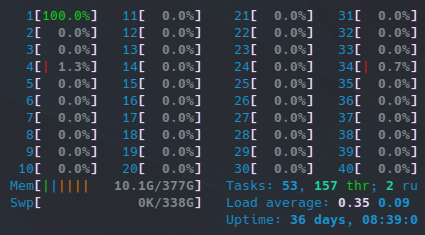
\includegraphics[width=\textwidth]{figures/htop_cpus/1CPU_1Thread.png}
        \caption{1 CPU, 1 Thread}\label{fig:1CPU_1Thread}
    \end{minipage}
    \hspace{0.4cm}
    \centering
    \captionsetup{width=.48\linewidth}
    \begin{minipage}[t]{0.48\textwidth}
        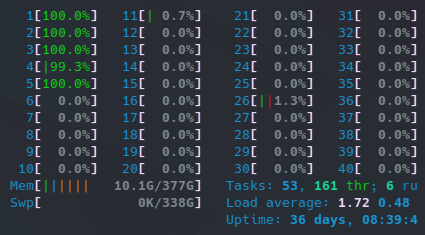
\includegraphics[width=\textwidth]{figures/htop_cpus/1CPU_5Threads.png}
        \caption{1 CPU, 5 Threads}\label{fig:1CPU_5Threads}
    \end{minipage}

% 1 CPU: 10 & 20 Threads
    \centering
    \captionsetup{width=.48\linewidth}
    \begin{minipage}[t]{0.48\textwidth}
        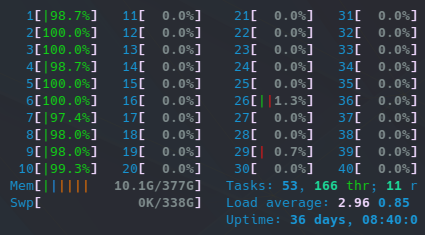
\includegraphics[width=\textwidth]{figures/htop_cpus/1CPU_10Threads.png}
        \caption{1 CPU, 10 Threads}\label{fig:1CPU_10Threads}
    \end{minipage}
    \hspace{0.4cm}
    \centering
    \captionsetup{width=.48\linewidth}
    \begin{minipage}[t]{0.48\textwidth}
        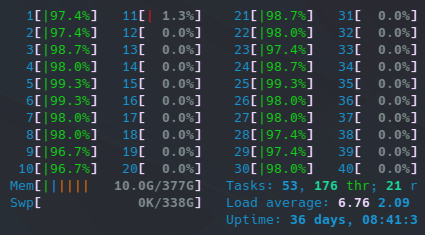
\includegraphics[width=\textwidth]{figures/htop_cpus/1CPU_20Threads.png}
        \caption{1 CPU, 20 Threads}\label{fig:1CPU_20Threads}
    \end{minipage}

% 2 CPUs: 2 & 10 Threads
    \centering
    \captionsetup{width=.48\linewidth}
    \begin{minipage}[t]{0.48\textwidth}
        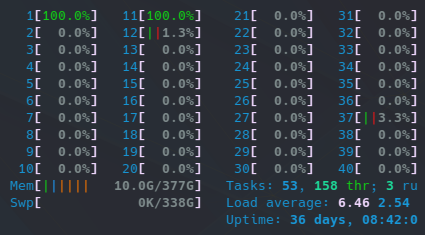
\includegraphics[width=\textwidth]{figures/htop_cpus/2CPUs_2Threads.png}
        \caption{2 CPUs, 2 Threads}\label{fig:2CPUs_2Threads}
    \end{minipage}
    \hspace{0.4cm}
    \centering
    \captionsetup{width=.48\linewidth}
    \begin{minipage}[t]{0.48\textwidth}
        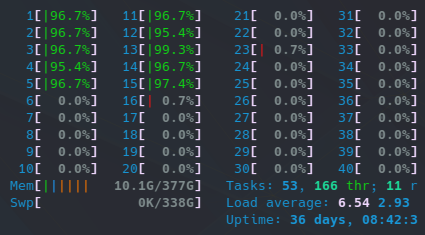
\includegraphics[width=\textwidth]{figures/htop_cpus/2CPUs_10Threads.png}
        \caption{2 CPUs, 10 Threads}\label{fig:2CPUs_10Threads}
    \end{minipage}

% 2 CPUs: 20 & 40 Threads
    \centering
    \captionsetup{width=.48\linewidth}
    \begin{minipage}[t]{0.48\textwidth}
        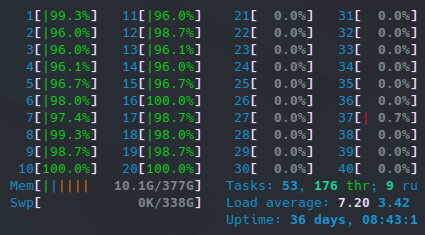
\includegraphics[width=\textwidth]{figures/htop_cpus/2CPUs_20Threads.png}
        \caption{2 CPUs, 20 Threads}\label{fig:2CPUs_20Threads}
    \end{minipage}
    \hspace{0.4cm}
    \centering
    \captionsetup{width=.48\linewidth}
    \begin{minipage}[t]{0.48\textwidth}
        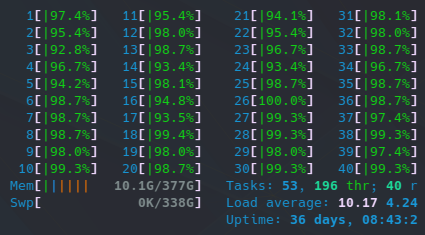
\includegraphics[width=\textwidth]{figures/htop_cpus/2CPUs_40Threads.png}
        \caption{2 CPUs, 40 Threads}\label{fig:2CPUs_40Threads}
    \end{minipage}
\end{figure*}

% 1 & 2 GPUs
\begin{figure*}[!h]
    \centering
    \captionsetup{width=.48\linewidth}
    \begin{minipage}[t]{0.48\textwidth}
        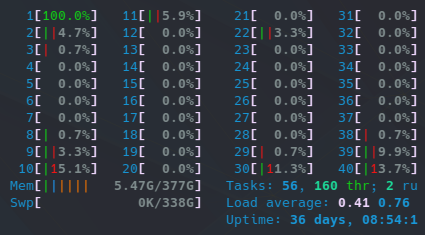
\includegraphics[width=\textwidth]{figures/htop_gpus/1GPU_1Thread.png}
        \caption{1 GPU, 1 Thread}\label{fig:1GPU_1Thread}
    \end{minipage}
    \hspace{0.4cm}
    \centering
    \captionsetup{width=.48\linewidth}
    \begin{minipage}[t]{0.48\textwidth}
        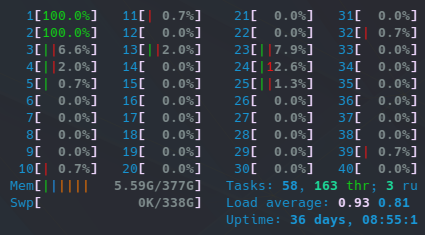
\includegraphics[width=\textwidth]{figures/htop_gpus/2GPUs_2Threads.png}
        \caption{2 GPUs, 2 Threads}\label{fig:2GPUs_2Threads}
    \end{minipage}

% 4 & 8 GPUs
    \centering
    \captionsetup{width=.48\linewidth}
    \begin{minipage}[t]{0.48\textwidth}
        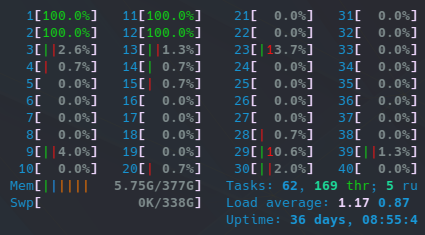
\includegraphics[width=\textwidth]{figures/htop_gpus/4GPUs_4Threads.png}
        \caption{4 GPUs, 4 Threads}\label{fig:4GPUs_4Threads}
    \end{minipage}
    \hspace{0.4cm}
    \centering
    \captionsetup{width=.48\linewidth}
    \begin{minipage}[t]{0.48\textwidth}
        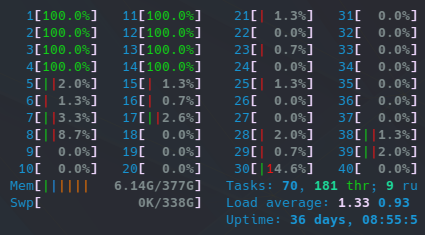
\includegraphics[width=\textwidth]{figures/htop_gpus/8GPUs_8Threads.png}
        \caption{8 GPUs, 8 Threads}\label{fig:8GPUs_8Threads}
    \end{minipage}

% 1 CPU, 4 Threads + 1 GPU, 1 Thread
% 1 CPU, 8 Threads + 2 GPUs, 2 Threads
    \centering
    \captionsetup{width=.48\linewidth}
    \begin{minipage}[t]{0.48\textwidth}
        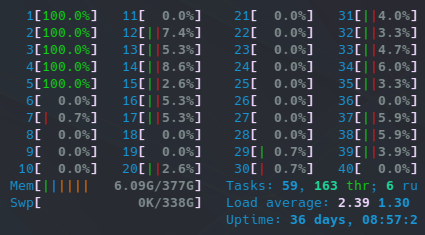
\includegraphics[width=\textwidth]{figures/htop_hybrid/1CPU_4Threads___1GPU_1Thread.png}
        \caption{1 CPU, 4 Threads + 1 GPU, 1 Thread}\label{fig:1CPU_4Threads___1GPU_1Thread}
    \end{minipage}
    \hspace{0.4cm}
    \centering
    \captionsetup{width=.48\linewidth}
    \begin{minipage}[t]{0.48\textwidth}
        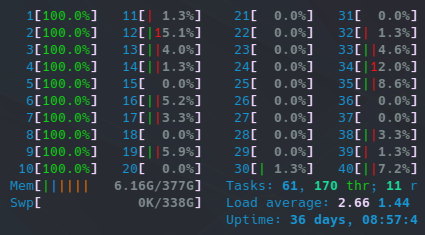
\includegraphics[width=\textwidth]{figures/htop_hybrid/1CPU_8Threads___2GPUs_2Threads.png}
        \caption{1 CPU, 8 Threads + 2 GPUs, 2 Threads}\label{fig:1CPU_8Threads___2GPUs_2Threads}
    \end{minipage}

% 2 CPUs, 16 Threads + 4 GPU, 4 Threads
% 2 CPUs, 32 Threads + 8 GPUs, 8 Threads
    \centering
    \captionsetup{width=.48\linewidth}
    \begin{minipage}[t]{0.48\textwidth}
        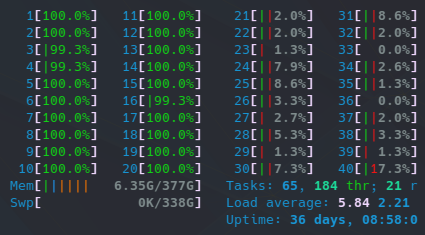
\includegraphics[width=\textwidth]{figures/htop_hybrid/2CPUs_16Threads___4GPUs_4Threads.png}
        \caption{2 CPUs, 16 Threads + 4 GPU, 4 Threads}\label{fig:2CPUs_16Threads___4GPUs_4Threads}
    \end{minipage}
    \hspace{0.4cm}
    \centering
    \captionsetup{width=.48\linewidth}
    \begin{minipage}[t]{0.48\textwidth}
        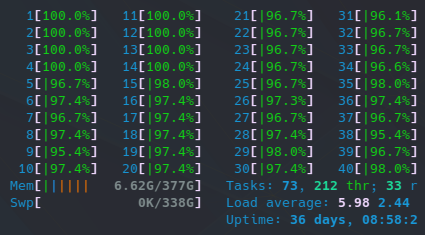
\includegraphics[width=\textwidth]{figures/htop_hybrid/2CPU_32Threads___8GPUs_8Threads.png}
        \caption{2 CPUs, 32 Threads + 8 GPUs, 8 Threads}\label{fig:2CPU_32Threads___8GPUs_8Threads}
    \end{minipage}
\end{figure*}

% =================================================================================================

% [IMPORTANT! ADD ONE BIG TREE, GIVING THE OVERVIEW ON ALL THE CONFIGS RELATIONS!]

% =================================================================================================

% \begin{itemize}
%     \item Server $-$ The tests will be conducted on two computational
%     nodes, that slightly differs from each other based on hardware equipped.
%         \begin{itemize}
%             \item sanna.kask
%             \item vinnana.kask
%         \end{itemize}
%     \item Device $-$ Next, benchmarks will be organized based on devices,
%     that will be utilized during tests.
%         \begin{itemize}
%             \item CPU\@(s)
%             \item GPU\@(s)
%             \item Hybrid (CPUs + GPUs)
%         \end{itemize}
%     \item Implementation $-$ Depending on current server, as well as device
%     chosen, the implementation technology is specified.
%         \begin{itemize}
%             \item OMP-CPP (sanna.kask, CPU\@(s))
%             \item OMP-CUDA (sanna.kask, GPU\@(s))
%             \item OMP-CPP + OMP-CUDA (sanna.kask, CPU\@(s) + GPU\@(s))
%             \item MPI-Fortran (vinnana.kask, CPU\@(s))
%             \item Horovod-Python (vinnana.kask, GPU\@(s))
%             \item MPI-Fortran + Horovod-Python (vinnana.kask, CPU\@(s) + GPU\@(s))
%         \end{itemize}
%     \item Benchmark and class size $-$ Picking the correct benchmark by the
%     automation scheduler is based on implementation technology currently
%     chosen as well device and server.
%         \begin{itemize}
%             \item OMP-CPP
%             \begin{itemize}
%                 \item bt.C
%                 \item is.D
%                 \item lu.C
%             \end{itemize}
%         \end{itemize}
%         \begin{itemize}
%             \item OMP-CUDA
%             \begin{itemize}
%                 \item lu.D
%                 \item sp.D
%                 \item ep.D
%             \end{itemize}
%         \end{itemize}
%         \begin{itemize}
%             \item Hybrid (OMP-CPP + OMP-CUDA)
%             \begin{itemize}
%                 \item bt.C+lu.D
%                 \item is.D+sp.D
%                 \item lu.D+ep.D
%             \end{itemize}
%         \end{itemize}
%         \begin{itemize}
%             \item MPI-Fortran
%             \begin{itemize}
%                 \item ep.D.x
%                 \item is.D.x
%                 \item lu.C.x
%             \end{itemize}
%         \end{itemize}
%         \begin{itemize}
%             \item Horovod-Python
%             \begin{itemize}
%                 \item XCeption
%             \end{itemize}
%         \end{itemize}
%         \begin{itemize}
%             \item Hybrid (MPI-Fortran + Horovod-Python)
%             \begin{itemize}
%                 \item ep.D.x+XCeption
%                 \item is.D.x+XCeption
%                 \item lu.C.x+XCeption
%             \end{itemize}
%         \end{itemize}
%     \item Configuration $-$ lastly, the configuration of number of logical
%     processors on CPU\@(s) and/or number of GPU\@(s) used in test are based on
%     chosen implementation.
%         \begin{itemize}
%             \item for OMP-CPP implementation:
%             \item 1 CPU 1 Thread
%             \item 1 CPU 5 Threads
%             \item 1 CPU 10 Threads
%             \item 1 CPU 20 Threads
%             \item 2 CPUs 2 Threads
%             \item 2 CPUs 10 Threads
%             \item 2 CPUs 20 Threads
%             \item 2 CPUs 40 Threads
%         \end{itemize}
%         \begin{itemize}
%             \item for OMP-CUDA implementation:
%             \item 1 GPU 1 Thread
%             \item 2 GPUs 2 Threads
%             \item 4 GPUs 4 Threads
%             \item 8 GPUs 8 Threads
%         \end{itemize}
%         \begin{itemize}
%             \item for OMP-CPP+OMP-CUDA implementation:
%             \item 1 CPU 4 Threads \& 1 GPU 1 Thread
%             \item 1 CPU 8 Threads \& 2 GPUs 2 Threads
%             \item 2 CPUs 16 Threads \& 4 GPUs 4 Threads
%             \item 2 CPUs 32 Threads \& 8 GPUs 8 Threads
%         \end{itemize}
%         \begin{itemize}
%             \item for MPI-Fortran implementation:
%             \item Processes: 4
%             \item Processes: 8
%             \item Processes: 16
%             \item Processes: 32
%         \end{itemize}
%         \begin{itemize}
%             \item for Horovod-Python implementation:
%             \item 1 GPU
%             \item 2 GPUs
%             \item 4 GPUs
%         \end{itemize}
%         \begin{itemize}
%             \item for MPI-Fortran+Horovod-Python implementation:
%             \item Processes: 8 \& 1 GPU
%             \item Processes: 16 \& 2 GPUs
%             \item Processes: 32 \& 4 GPUs
%         \end{itemize}
% \end{itemize}


